% -----
% ARQUIVO: capitulo-05.tex
% VERSÃO: 1.0
% DATA: Agosto de 2015
%
% CAPÍTULO DE PLANO DE AÇÃO DA PROPOSTA
%
% NÃO MEXA NAS SEÇÕES, SOMENTE EDITE O CONTEÚDO.
% -----

\chapter{Plano de A\c{c}\~{a}o}
% #TXT_PLANO
\lipsum[1]

\section{Metodologia}
% #TXT_METODOLOGIA
\lipsum[11]

% Para usar tabelas, use sempre o mesmo template abaixo. Altere somente:
% 1. \caption{*} / para colocar o rótulo da tabela em *
% 2. \begin{tabular}{*} / para colocar a formatação da tabela em *
% 3. o conteúdo da tabela (tudo até \end{tabular})

\begin{table}[h]
\centering
\caption{Um nome qualquer}
\vspace{0.5cm}
\begin{tabular}{r|lr}
 
Posi\c{c}\~ao & Pa\'is & IDH \\ % Note a separação de col. e a quebra de linhas
\hline                               % para uma linha horizontal
1 & Noruega        & .955 \\
2 & Austr{\'a}lia  & .938 \\
3 & EUA            & .937 \\
4 & Holanda        & .921 \\
5 & Alemanha       & .920            % não é preciso quebrar a última linha
 
\label{tab:tabela1}
\end{tabular}
\end{table}

At vero eos et accusamus et iusto odio dignissimos ducimus qui blanditiis praesentium voluptatum deleniti atque corrupti quos dolores et quas molestias excepturi sint occaecati cupiditate non provident, similique sunt in culpa qui officia deserunt mollitia animi, id est laborum et dolorum fuga (como mostrado na Tabela \ref{tab:tabela1}). Et harum quidem rerum facilis est et expedita distinctio. Nam libero tempore, cum soluta nobis est eligendi optio cumque nihil impedit quo minus id quod maxime placeat facere possimus, omnis voluptas assumenda est, omnis dolor repellendus. Temporibus autem quibusdam et aut officiis debitis aut rerum necessitatibus saepe eveniet ut et voluptates repudiandae sint et molestiae non recusandae.

\section{Cronograma}
\lipsum[11]

O cronograma para o desenvolvimento das atividades relacionadas a esta proposta pode ser visto na Figura \ref{fig:cronograma}.

% Para usar figuras, use sempre o mesmo template abaixo. altere somente:
% 1. os parâmetros do comando \includegraphics[width=•]{•} / tamanho e arquivo
% 2. \caption{*} / para colocar o rótulo da figura em *
% 3. \label{*} / para colocar a chamada para a figura no texto em *
%    TODA figura deve ter uma chamada no texto e esta deve ser feita sempre no formato:
%    Figura \ref{•} (p. ex. "Figura \ref{fig:cronograma}")

% #CRONOGRAMA
\begin{figure}[!h]
	\centering
	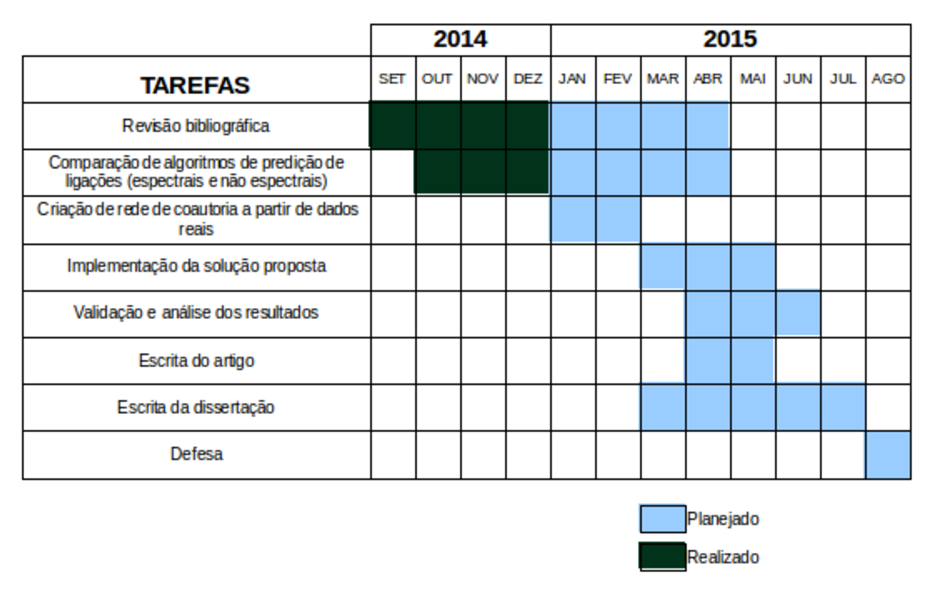
\includegraphics[width=0.9\textwidth]{cronograma.eps}
	\caption{Cronograma da Proposta de Disserta\c{c}\~{a}o.}
	\label{fig:cronograma}
\end{figure}


